\q{15}{Sampling}

Assume you are given the following Bayes’ net and the corresponding distributions over the variables in the Bayes’ net.

\begin{tabular}{c c c c c}
\parbox[c]{4cm}{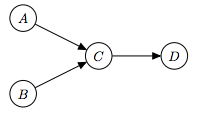
\includegraphics[width =1.5\linewidth]{figs/sampling_graph.png}}
\hspace{2cm}
\begin{tabular}{|c |c|}
\hline
\multicolumn{2}{|c|}{$P(A)$} \\
\hline
t & $0.1$\\
\hline
\end{tabular}
&
\begin{tabular}{|c | c|}
\hline
\multicolumn{2}{|c|}{$P(B)$} \\
\hline
t & .7 \\
\hline
\end{tabular}
&
\begin{tabular}{| c | c | c | c |}
\hline
$A$ & $B$ & $P(C = t | A, B)$\\
\hline
t & t & .25\\
\hline
f & t & .6\\
\hline
t & f & .5\\
\hline
f & f & .2\\
\hline
\end{tabular}
&
\begin{tabular}{| c | c | c |}
\hline
$C$ & $P(D = t |C)$\\
\hline
t & .5\\
\hline
f & .8\\
\hline
\end{tabular}
\end{tabular}



\begin{question}{}
  [4 pts] Assume we receive evidence that A = t. If we were to draw samples using rejection sampling, on
 expectation what percentage of the samples will be rejected?
\end{question}
\begin{minipage}{\textwidth}
\qquad \qquad \textbf{90\%}
\end{minipage}
\vspace{1.5cm}

\begin{question}{}
  [3 pts] Next, assume we observed both A = t and D = t. What are the weights for the following samples
 under likelihood weighting sampling?
\begin{center}
\begin{tabular}{|c|c|}
\hline
 Sample & Weight  \\
 \hline
 $(A=t,B=f,C=t,D=t)$ & $0.05$\\
 \hline
 $(A=t,B=f,C=f,D=t)$ & $0.08$\\
 \hline
 $(A=t,B=t,C=f,D=t)$ & $0.08$\\
 \hline
\end{tabular}
\end{center}
\end{question}


\begin{question}{}
  [4 pts] Given the samples in the previous question, estimate $P(B=f| A=t, D=t)$.
\end{question}
\begin{minipage}{\textwidth}
\qquad \qquad $P(B=f|A=t,D=t) \approx \frac{0.05+0.08}{0.05+0.08+0.08} = 0.619$
\end{minipage}
\vspace{1.5cm}

\begin{question}{}
  [4 pts] Assume we need to (approximately) answer two different inference queries for this graph: $P(C| A=t)$
and $P(C| D=t)$. You are required to answer one query using likelihood weighting and one query using Gibbs
sampling. In each case you can only collect a relatively small amount of samples, so for maximal accuracy
you need to make sure you cleverly assign algorithm to query based on how well the algorithm fits the query.
Which query would you answer with each algorithm?

\begin{table}[h]
\centering
\begin{tabular}{cc}

\begin{tabular}{|c|c|}
\hline
Algorithm & \ \ \ \ \ \ \ \ \ Query \ \ \ \ \ \ \ \ \ \\
\hline
& \\
Likelihood Weighting & $P(C|A=t)$
\\
& \\
\hline
\end{tabular}
&
\begin{tabular}{|c|c|}
\hline
Algorithm & \ \ \ \ \ \ \ \ \ Query \ \ \ \ \ \ \ \ \ \\
\hline
& \\
Gibbs Sampling & $P(C|D=t)$
\\
& \\
\hline
\end{tabular}
\end{tabular}
\end{table}

\begin{minipage}{\textwidth}
Justify your answer:
\end{minipage}
If you sample for $P(C|A=t)$ using likelihood waiting, all samples will have equal weight of $0.1$ because $A$ has no parents. This makes it more accurate because it essentially reduces the problem by eliminating variable $A$ and asking what is $P(C)$.

\end{question}







